\documentclass[draft]{book}
\newcommand{\docversion}{0.181}

% Needed so characters such as underscore are recognized in PDF
% viewers. Otherwise searching for say `hsa_open` produces no
% results
\usepackage[T1]{fontenc}

% If draft, use narrow margins (better for printing)
\usepackage{ifdraft}
\ifdraft{\usepackage[top=.5cm,bottom=.5cm,left=.5cm,right=.5cm]{geometry}}
         {\usepackage[top=2.5cm,bottom=2.5cm,left=2.5cm,right=2.5cm]{geometry}}
%\usepackage[top=2.5cm,bottom=2.5cm,left=2.5cm,right=2.5cm]{geometry}

\usepackage[toc,page]{appendix}
\usepackage[usenames,dvipsnames,svgnames,table]{xcolor}
  \definecolor{lightgray}{gray}{0.9}
\usepackage{makeidx}
\usepackage[final]{graphicx}
\usepackage{sidecap}
\usepackage{float}

% overwrite global draft option so the source is shown in draft mode
\usepackage[final]{listings}

% allow tables across page breaks
\usepackage{longtable}

% Use Tikz for simple diagrams
\usepackage{tikz}
\usetikzlibrary{arrows,automata,positioning,chains}
\tikzset{
    % define global arrow tip format
    >=angle 45}

% allows width arithmetic, currently used in the LaTeX generated by xml2py
\usepackage{calc}
% allow usage of underscore w/o resorting to underscore package
% the underscore package imposes more restrictions on where underscores still
% cannot be used (e.g.: labels)
\catcode`\_=12

\usepackage{ifthen}
\usepackage{textcomp}
\usepackage{paralist}
\usepackage{framed}
\usepackage{times}
\usepackage[titles]{tocloft}
\usepackage{fancyhdr}
\usepackage{enumitem}

% colored boxes with plenty of configuration properties
\usepackage{tcolorbox}
  % allow page breaks within boxes
  \tcbuselibrary{breakable}

\usepackage{ifpdf}
\ifpdf
\usepackage[pdftex,
            bookmarks,
            final, % use links even if the document is draft
            pagebackref=true,
            pdfpagemode=UseOutlines, % generate index
            linktoc=all,  % sections and subsections linked
            colorlinks=true,
            linkcolor=black,
            unicode
           ]{hyperref}
\else
\usepackage[ps2pdf,
            bookmarks,
            final, % use links even if the document is draft
            pdfpagemode=UseOutlines, % generate index
            linktoc=all,  % sections and subsections linked
            pagebackref=true,
            colorlinks=true,
            linkcolor=black,
            unicode
           ]{hyperref}
\usepackage{pspicture}
\fi

\lstset{language=C++,
        inputencoding=utf8,
        basicstyle=\small,
        breaklines=true,
        breakatwhitespace=true,
        tabsize=4,
        showstringspaces=false,
        frame=none,
        backgroundcolor=\color{lightgray},
        keywordstyle=,
        emphstyle={\textbf},
        commentstyle=\color{ForestGreen},
        morecomment=[l][\color{green}]{\#}
}
% include automatically-generated Listing commands
\input{api/altlatex/listings}

% formatting of arguments, function names, types, etc.
% remember to add this commands to the safe command list of Latexdiff so
% it includes them in the diff algorithm
\newcommand{\hsaarg}[1]{\textit{#1}}
\newcommand{\reffun}[1]{\textbf{#1}}
\newcommand{\refarg}[1]{\textit{#1}}
\newcommand{\reffld}[1]{\textit{#1}}
\newcommand{\reftyp}[1]{#1}
\newcommand{\refenu}[1]{\reftyp{#1}}
\newcommand{\refhsl}[1]{\reffun{#1}}

\usepackage{pdftexcmds}
\input{api/altlatex/commands}

% every section in a new page
\usepackage{etoolbox}
\pretocmd{\section}{%
  \ifnum\value{section}=0 \else\clearpage\fi
}{}{}

% define marginparwidth so todonotes renders properly
\setlength{\marginparwidth}{2cm}
\usepackage[obeyDraft,obeyFinal,textsize=scriptsize]{todonotes}

%%%%%%%%%%%%%%%%%%%%%%%%%%%%%%%%%%%%%%%%%%%%%%%%%

% push footer a little further away
\setlength{\footskip}{35pt}

% Side notes. One command per author
\newcommand{\mariotodo}[1]{\todo[color=CarnationPink]{#1}}

% Increase paragraph separation
\setlength{\parskip}{2mm}

% no indentation
\setlength{\parindent}{0cm}

% number (sub)sections up to level 3
\setcounter{secnumdepth}{3}

\makeindex
\setcounter{tocdepth}{3}
\renewcommand{\footrulewidth}{0.4pt}
\renewcommand{\familydefault}{\sfdefault}

\RequirePackage[normalem]{ulem} %DIF PREAMBLE
\newenvironment{DIFnomarkup}{}{}

% header and footer layout
\pagestyle{fancy}
\renewcommand{\chaptermark}[1]{ \markboth{#1}{} }
\renewcommand{\sectionmark}[1]{ \markright{#1}{} }
\renewcommand{\headrulewidth}{0pt}
\renewcommand{\footrulewidth}{0pt}
\fancyhead{} % clear all header fields
\fancyfoot{} % clear all footer fields
\fancyfoot[LE,RO]{\scriptsize{\thepage}}
\fancyfoot[LO,RE]{\scriptsize{HSA Runtime Programming Guide and API Reference v\docversion $\:$-$\:$\today}}
\fancyhead[RE]{\scriptsize{\leftmark}}
\fancyhead[LO]{\scriptsize{\rightmark}}


\begin{document}

\hypersetup{pageanchor=false,citecolor=black}
\begin{titlepage}

\includegraphics[width=.5\textwidth]{fig/foundation.png}
\vspace*{7cm}
\begin{center}
{\Large HSA Core API Programmers Reference Manual\\[1ex]\large\docversion}\\
\vspace*{1cm}
\vspace*{0.5cm}
{\small \today}\\
\vspace*{0.5cm}
{\small Draft}\\
\end{center}
\end{titlepage}
\thispagestyle{empty} {\textcopyright 2013-2014 HSA Foundation. All rights
  reserved.}


The contents of this document are provided in connection with the HSA Foundation
specifications. This specification is protected by copyright laws and contains
material proprietary to the HSA Foundation. It or any components may not be
reproduced, republished, distributed, transmitted, displayed, broadcast or
otherwise exploited in any manner without the express prior written permission
of HSA Foundation. You may use this specification for implementing the
functionality therein, without altering or removing any trademark, copyright or
other notice from the specification, but the receipt or possession of this
specification does not convey any rights to reproduce, disclose, or distribute
its contents, or to manufacture, use, or sell anything that it may describe, in
whole or in part.

HSA Foundation grants express permission to any current Founder, Promoter,
Supporter Contributor, Academic or Associate member of HSA Foundation to copy
and redistribute UNMODIFIED versions of this specification in any fashion,
provided that NO CHARGE is made for the specification and the latest available
update of the specification for any version of the API is used whenever
possible. Such distributed specification may be re-formatted AS LONG AS the
contents of the specification are not changed in any way. The specification may
be incorporated into a product that is sold as long as such product includes
significant independent work developed by the seller. A link to the current
version of this specification on the HSA Foundation web-site should be included
whenever possible with specification distributions.

HSA Foundation makes no, and expressly disclaims any, representations or
warranties, express or implied, regarding this specification, including, without
limitation, any implied warranties of merchantability or fitness for a
particular purpose or non-infringement of any intellectual property. HSA
Foundation makes no, and expressly disclaims any, warranties, express or
implied, regarding the correctness, accuracy, completeness, timeliness, and
reliability of the specification. Under no circumstances will the HSA
Foundation, or any of its Founders, Promoters, Supporters, Academic,
Contributors, and Associates members or their respective partners, officers,
directors, employees, agents or representatives be liable for any damages,
whether direct, indirect, special or consequential damages for lost revenues,
lost profits, or otherwise, arising from or in connection with these materials.

\clearpage \pagenumbering{roman}
\addtocontents{toc}{}
\tableofcontents
\clearpage

\pagenumbering{arabic}
\setcounter{page}{1}

\chapter{Introduction} \label{index}\hypertarget{index}{}
\hypertarget{overview}{}\section{Overview}\label{overview}

Recent system-on-a-chip designs have integrated CPU, GPU, and other accelerator
devices onto a single chip with a shared high-bandwidth memory system. In fact,
these single-chip designs are now widely used in many computing markets
including cellphones, tablets, personal computers, and game consoles. The
Heterogeneous System Architecture (HSA) builds on the close physical integration
of accelerators that is already occurring in the marketplace, and takes the next
step by defining standards for uniting the accelerators architecturally. The
HSA specifications includes requirements for virtual memory, memory coherency,
architected dispatch mechanisms, and power-efficient signals. HSA refers to
these accelerators as "components". The system architecture defines a
consistent base for building portable applications that access the power and
performance benefits of the dedicated HSA components. Many of these components,
including GPUs and DSPs, are capable and flexible processors that have been
extended with special hardware for accelerating parallel code. Historically
these devices have been difficult to program due to a need for specialized or
proprietary programming languages. HSA aims to bring the benefits of these
components to mainstream programming languages using similar or identical syntax
to that which is provided for accessing multi-core CPUs.

In addition to the system architecture, HSA's "Programmer's Reference Guide"
defines HSAIL - a portable, low-level, compiler intermediate language designed
for parallel computing.

\begin{description}
\item[Portable:] The HSAIL language is an open-standard, supported by multiple
  vendors in the HSA Foundation, and is portable across vendors and product
  generations, so that applications which use HSAIL are guaranteed to run on
  future hardware that supports the HSAIL standard.
\item[Low-level:] HSAIL's representation is just above the machine instruction
  set. Most optimizations including register allocation are intended to be
  performed by the compiler that generates HSAIL. HSAIL code is translated to
  the host instruction set by a tool called the "finalizer". Each component
  will provide its own implementation of the finalizer. The finalization step
  is intended to be lightweight, fast, and simple. Importantly, the finalizer
  step does not involve a complex compiler. Applications which contain HSAIL
  should not see different functional or performance behavior from new finalizer
  versions that might be deployed in the field after the application ships.
\item[Designed for parallel computing:] HSAIL is intended to represent the
  parallel sections of an application. It complements but does not replace the
  host code – host code still exists and is used for the serial portion of the
  application. HSAIL represents a single "lane" of execution, and the
  parallelism is expressed in the grid dimensions that are specified when the
  HSAIL kernel is dispatched to a target component. In this way, HSAIL does not
  encode a specific "vector width" and can be used to represent a variety of
  different parallel computing devices.
\end{description}

For more information on HSAIL, refer to the HSA Programmer's Reference Guide.

The final piece of the puzzle is the HSA Core Runtime API. The core runtime is
a thin, user-mode API that provides the interfaces necessary for the host to
launch compute kernels to the available components. This document describes the
architecture and APIs for the HSA Core Runtime. Key sections of the runtime API
include:
\begin{itemize}
\item Error handling
\item Runtime initialization (open/close)
\item Topology Discovery
\item Signals and Synchronization
\item Architected Dispatch
\item Memory Management
\end{itemize}
In summary, there are three specifications provided by the HSA
Foundation:
\begin{description}
\item[HSA System Architecture Requirements:] Architectural foundation for
how HSA components share memory and communicate work requests.
\item[HSA Programmer's Reference Manual:] Describes HSAIL, a low-level,
portable compiler IR appropriate for use as compiler intermediate
language.
\item[HSA Runtime Specification:] This document. Describes the host-side
API for controlling the launch of HSAIL kernels.
\end{description}

The remainder of this document describes the HSA software architecture and
execution model, and includes functional descriptions for all of the HSA APIs
and associated data structures.

\begin{figure}
  \centering
  \tikzstyle{lang}=[rectangle,draw,fill=black!30,align=center,minimum width=1.25cm,minimum height=.75cm]
  \tikzstyle{hsa}=[rectangle,draw,fill=black!10,align=center,minimum height=.75cm]
  \tikzstyle{comp}=[rectangle,draw,minimum height=.75cm]
  \begin{tikzpicture}[thick,auto, node distance=1.5cm]
    \scriptsize
    \node[lang] (l0) {OpenCL\texttrademark \\ app};
    \node[lang,below of=l0] (r0) {OpenCL\texttrademark \\ runtime};

    \node[lang,right of=l0] (l1) {Java \\ app};
    \node[lang,below of=l1] (r1) {JVM};

    \node[inner sep=0,below right=.75cm of l1] (k) {...};

    \node[lang,above right=.75cm of k] (l2) {OpenMP \\ app};
    \node[lang,below of=l2] (r2) {OpenMP \\ runtime};

    \node[lang,right of=l2] (l3) {DSL \\ app};
    \node[lang,below of=l3] (r3) {DSL \\ runtime};

    \node[hsa,minimum width=3.5cm,below=2cm of k] (h) {HSA runtime};
    \node[hsa,minimum width=3cm,right=1.5cm of h] (hf) {HSA finalizer};
    \tiny
    \node[comp, below=.75cm of h.west,anchor=west] (c1) {HSA component 1};
    \node[below=.5cm of h.south,anchor=south]       (cAny)  {...};
    \node[comp,below=.75cm of h.east,anchor=east]  (cN) {HSA component N};

    \path[->]
       (l0) edge (r0)
       (l1) edge (r1)
       (l2) edge (r2)
       (l3) edge (r3)
       (r0.south) edge (h)
       (r1) edge (h)
       (r2) edge (h)
       (r3.south) edge (h)
       (h) edge[dashed] (hf)
    ;
  \end{tikzpicture}
  \caption{HSA Software Architecture}
  \label{fig:swarch}
\end{figure}

Figure~\ref{fig:swarch} shows how the HSA Core Runtime fits into a
typical software architecture stack.

At the top of the stack is a programming model such as OpenCL\texttrademark,
Java, OpenMP, or a domain-specific language (DSL). The programming model must
include some way to indicate a parallel region that can be accelerated. For
example, OpenCL has calls to \texttt{clEnqueueNDRangeKernel} with associated
kernels and grid ranges. Java has the stream and lambda APIs, which provide
support for both multi-core CPUs and HSA Components. OpenMP contains OMP pragmas
that mark parallel for loops and control other aspects of the parallel
implementation.  Other programming models can also build on this same
infrastructure.

The language compiler is responsible for generating HSAIL code for the parallel
regions. HSA supports several options for when HSAIL is generated and
finalized. One possibility is that the HSAIL is generated by a high-level
compiler and then embedded in the application binary. In this case, the
finalizer is run when the application loads and will convert the HSAIL to
machine code for the target machine. Another option is that the HSAIL is
finalized when the applications is built, or the machine cod The HSA Finalizer
is an optional component of the HSA Core Runtime, which may reduce the footprint
of the HSA software on systems where the finalization is done before runtime.

Each language also includes a "language runtime" that connects the language
implementation to the HSA Core Runtime. When the language compiler generates
code for a parallel region, it will include calls to the HSA Runtime to set up
and dispatch the work to the HSA Component. The language runtime is also
responsible for initializing HSA, and may utilize other HSA core runtime
features as well.

The API for the HSA core runtime is standard across all HSA vendors, such that
languages which use the HSA runtime can run on the different vendors that
support the API. Each vendor is responsible for supplying their own
implementation which supports the HSA component(s) in the vendor's platform. HSA
does not provide a mechanism to combine runtimes from different vendors; instead
vendors must provide a single runtime which supports all the components in the
platform. The implementation of the HSA Runtime may include kernel-level
components (typical for hardware components) or may be entirely user-space
(simulators or CPU implementations).

\hypertarget{executionmodel}{}\section{Execution
Model}\label{executionmodel}


\hypertarget{archdispatch}{}\subsection{Architected Dispatch}
\label{archdispatch}

Core runtime exposes several details of the HSA hardware, including architected
dispatches and support for execution control. The overall goal of the core
runtime design is to provide a high-\/performance dispatch mechanism that is
portable across multiple HSA vendor architectures. Two vendors with the same
host ISA but different HSA-\/compliant GPUs will be able to run the same
unmodified binary, because they support the HSA-\/architected AQL interface and
supply a library that implements the architected core runtime API.

In order for user-level applications to use the HSA system and HSA components,
they need to write HSAIL programs and compile and execute these programs using
user mode queues and AQL commands. The HSA Programmer's Reference Manual (PRM)
defines HSAIL Virtual ISA and Programming Model, serves as a Compiler Writer's
Guide, and defines Object Format (BRIG). The HSA runtime helps setup the
execution via API calls and data structures to support architected features.

The HSA core runtime realizes architected dispatch. Architected dispatch is the
key feature in an HSA system that enables a user-\/level application to directly
issue commands to the HSA Component hardware. Architected dispatch
differentiates it from other higher-\/level runtime systems and programming
models: other runtime systems provide software APIs for setting arguments and
launching kernels, while HSA architects these at the hardware and specification
level. The critical path of the dispatch mechanism is architected at the HSA
hardware level and can be done with regular memory operations and runtime
provided wrapper API. Fundamentally, the user creates user mode queues and an
AQL Packet in memory, and then signals the HSA component to begin executing the
packet using light weight operations (which may be wrapped with API calls).

This section describes various features core runtime provides to support
architected dispatch as steps that a user needs to take to utilize runtime.

\subsection{Initial Setup}
One of the first steps in the setup is that of device discovery. Device
discovery is performed at the initialization of the core runtime and information
is made available to the user as data structures. Section~\ref{topology}
describes these structures. The next step in the setup is creation of the
component queues. Queues are an HSA architected mechanism to submit work to the
HSA component HW. The interfaces for queue creation are defined in
Section~\ref{architected-queue}. Different components may provide
implementation-\/specific code under the core API for these functions. HSA
runtime also includes mechanisms to provide implementation-\/specific data as
part of the dispatch, provided such data can be computed at compile time.

\subsection{Compilation Flow}
Once an HSAIL program is written or generated by a higher-level compilation
step, it needs to be \emph{assembled} to generate a BRIG. BRIG is the HSAIL
object format and is specified in the PRM. HSA runtime defines API call to
compile the BRIG and generate a code object that has sufficient information to
execute the user program. The details of this compilation process and symbol
resolution are discussed in Section~\ref{finalizerchapter}.

\subsection{Execution of Kernel}
The Systems Architecture Requirements (SAR) document specifies the structure of
the \emph{packets} (i.e. commands) that can be placed on the HSA user mode
queues for the component HW to execute them. The format of the packets is
architected and they are referred to as Architected Queuing Language (AQL)
packets. One of the types of AQL packets is a dispatch AQL packet. The user can
now create an AQL packet and initialize it with the code object obtained from
the finalization step, including the allocation of memory to hold the kernel
arguments and the spill/arg/private memory. The interface for kernel arguments
between the runtime and the kernel ISA (instruction set architecture) is also
architected at the HSA level. This is covered in the HSAIL ABI, which specifies
the in-memory layout of the kernarg segment. Users can determine the layout of
the kernarg memory segment at compile time merely by examining the signature of
the HSAIL function. The finalizer is required to support this ABI and thus there
is no need for runtime metadata to specify the position or format of arguments.
This step can be done once for each AQL packet creation.

Optimized implementations can cache the result of this step and re-use the AQL
packet for subsequent launches. Care must be taken to ensure that the AQL
Dispatch packet (and the associated kernel and spill/arg/private memory) is not
re-used before the launch completes. For simple cases, (that is, a
single-thread, synchronous launch, the AQL dispatch packet(s) can be declared
as a static variable and initialized at the same time the code is
finalized. More advanced cases can create and track several AQL Dispatch
packet(s) for a single kernel code object.

HSA HW defines a packet process for processing these packets and a doorbell
mechanism to inform the packet processing HW that packets have been written into
the queue. The Core runtime defines a structure and update API to inform the HW
that the dispatch packet has been written to the queue. Different packet formats
and states of a packet are discussed in
Section~\ref{AQL}. Section~\ref{architected-queue} discusses the queue creation
and various states the queue can be in, once it is created.

Once the packet is written and the HW is informed by way of the doorbell, the
execution can start. The execution happens asynchronously. The user is free to
write more packets for executing other kernels in the queue. This activity can
overlap the actual execution of the kernel.

\subsection{Determining Kernel Completion}
HSA SAR defines signals as a mechanism for communication between different parts
of a HSA system. Signals are defined as opaque objects in the HSA core runtime
and APIs have been defined to send a value to the signal and wait for a value at
the signal, Section~\ref{signals} discusses signals in detail. The AQL dispatch
packet has a provision for the user to pass in an opaque signal. When the HSA
Component HW observes a valid signal in the AQL packet, it sends a value to this
signal when execution of the kernel is complete (success or error). The user can
wait on this signal to determine kernel completion. Errors and their meaning are
discussed in Section~\ref{error}.

\lstinputlisting{example/main.c}

\chapter{HSA Core Programming Guide} \label{coreapi}

\mariotodo{Surreal intro}This chapter describes HSA Core runtime API by their
functional area. Note that except for any setter/getter API, the remainder of
the core runtime API may be considered thread-safe. Both the signal update and
the queue index update API are setter/getter API and define scope an
synchronization that applies to the updates and operate on structure elements.

Several operating systems allow functions to be executed when a DLL or a shared
library is loaded (e.g. DLL main in Windows and GCC
\emph{constructor/destructor} attributes that allow functions to be executed
prior to main in several operating systems). Whether or not the HSA runtime
functions are allowed to be invoked in such fashion may be implementation
specific and are outside the scope of this specification.

Similarly, any header files distributed by the HSA foundation for this spec may
contain calling convention specific prefixes such as __cdecl or
__stdcall. Such calling conventions are again invocation, usage and
implementation specific. Hence, the calling convention specific prefix
definition is outside the scope of API definition.

\section{Initialization and Shutdown}\label{init}

Since the HSA core runtime is a user mode library, its state is a part of the
application's process space. When the runtime is opened for the first time, a
runtime instance for that application process is created. Closing a runtime
destroys this instance. An application may open (or close) the HSA runtime
multiple times within the same process and potentially within multiple threads
-- only a single instance of the runtime will exist for a given process.

The core runtime defines a runtime context that acts as a reference counting
mechanism and a scheme to differentiate multiple usages of the runtime within
the same application process. The runtime context is generated when the runtime
is opened or when a user calls the acquire API that is defined in this
Section. As an example, consider an application that is using the runtime but
also uses a library, this library also creates HSA queues and submits work to
them. Both the library and the application may want to register callbacks, and
to capture notifications/errors of their specific usage. The runtime context
helps identify the different usages (within the same process) and channel errors
and notifications to appropriate callbacks. It also acts as a reference counting
mechanism; while correctly acquired, the runtime context ensures that
the runtime instance will not be shutdown until the context is released
(this, in effect, is the reference counting part of the context).

\subsection{Example}
\lstinputlisting{example/openclose.c}

\section{Errors and Notifications}
\label{error}

Errors reported by the runtime can be synchronous or asynchronous. Synchronous
errors are always reported when the call returns. They indicate if the API
returned a success or an error. Asynchronous errors can occur due to various
reasons:\begin{inparaenum}[(i)]
\item Activity in packet processor, executing kernels, their actions and memory
  accesses. If an error is detected during execution of a kernel, the completion
  signal (if present) will be signaled with an error indication value.
\item To provide \textit{information/warning} (not as an exception in expected
  behavior but by definition). This information/warning may not necessarily
  indicate an error. For example, a timeout may be an acceptable response for a
  wait API but is not indicative of a failure.
\end{inparaenum}

\hypertarget{syncerror}{}\subsection{Synchronous Errors }\label{syncerror}

When a core runtime API is called by the user and does not execute successfully,
the core runtime returns a status that can help determine a cause of the
unsuccessful execution. Each API call discussed in this chapter defines what
constitutes a successful execution. While a few error conditions can be
generalized to a certain degree (e.g. failure in allocating system memory) many
errors can have system/implementation specific explanations.

The HSA core runtime API defines an enumeration that captures the result of any
API function that has been executed (the only exception to this behavior are
setter/getter API that access core runtime structures). This enumeration is of
the type \hsaref{hsa_status_t} and enumerates \textit{success}, \textit{info},
and \textit{error}. The \textit{info} status definition is discussed in
Section~\ref{asyncerror}.

\textit{Success} status is a single constant, \hsaref{HSA_STATUS_SUCCESS},
with value 0. Description of every core runtime API call that returns
\hsaref{hsa_status_t} explains the expected successful behavior for that API.

\textit{Error} status could be due to user input/actions that are not allowed
(e.g. negative value in a size for allocation) or systemic errors (e.g. an
asynchronous activity lead to a failure that cascaded into a failure in this
API). The constants used for error status are restricted to the negative range
of values within the \hsaref{hsa_status_t} enumeration. The name of any constant
that indicates an error status is prefixed by \refenu{HSA_STATUS_ERROR}.

While the name of the constant in itself is informative for success, info or
error status, there may be scenarios where\begin{inparaenum}[(i)]\item the user
  may request more information about the meaning of a particular status,
  or, \item the return status was implementation specific and the user needs to
  decode it.
\end{inparaenum} In the case of implementation specific status, the negative
number returned for error may not correspond to a particular enumeration
constant. To query additional information on synchronous errors, the core
runtime provides the \hsaref{hsa_status_query_description} API.

\hypertarget{asyncerror}{}\subsection{Asynchronous Errors and
Notifications}\label{asyncerror}

The HSA core runtime supports user-defined callbacks to handle asynchronous
errors. There are two different \mariotodo{why separating them?} categories of
callbacks that can be registered by the user:\begin{inparaenum}[(i)]\item for
  asynchronous information or warnings generated when the runtime is executing,
  or, \item for asynchronous errors that get generated in packet processor, or
  while executing a kernel \end{inparaenum}. The core runtime supports a
callback each for asynchronous errors and notifications. The user must use
caution when using blocking functions within their callback implementation -- a
callback that does not return can render the runtime state to be undefined. The
user cannot depend on thread local storage within the callbacks implementation
and may safely kill the thread that registers the callback. It is the user's
responsibility to ensure that the callback function is thread-safe. The runtime
does not implement any default callbacks.

The information/warning status is represented by a value greater than 0 within
the \hsaref{hsa_status_t} enumeration. The status is up to user interpretation
and the runtime allows the user to register a callback to take necessary
action. Consider the example where a user calls the initialize API to initialize
the core runtime and the return status is
\hsaref{HSA_STATUS_ALREADY_INITIALIZED} (to indicate that the core
runtime has already been initialized). This result may be interpreted
differently in different usage scenarios. A callback for such notifications may
be registered via \hsaref{hsa_open} API discussed in Section~\ref{init} or via
\hsaref{hsa_notification_callback_register} API.

The HSA system can have several queues in operation and several kernels
executing from these queues asynchronously. When any asynchronous activity
generates an error, the action that initiated the activity may have
concluded. To deal with asynchronous errors, the core runtime supports
asynchronous error callbacks. The asynchronous error callback may be registered
by means of the \hsaref{hsa_open} API discussed in Section~\ref{init} or via
\hsaref{hsa_error_callback_register} API.

\subsection{Asynchronous Notification Example}
\lstinputlisting{example/asyncerror.c}

\hypertarget{component}{}\section{Topology Discovery}
\label{topology}

Topology discovery is provided by the runtime so users can programmatically
query information about the available agents, memories, etc. This information
could be utilized by the user in different ways, including decisions on where to
execute a particular task. The runtime specification defines the topology table
data structure and other data structures to represent topology hierarchy.

A copy of the topology information can be created using
\hsaref{hsa_topology_table_create} after the runtime has been
initialized. The user can parse this table representing the HSA system to gather
details such as the number of different agents on the system with local access
to a particular set of memory resources. The topology table is designed to be
allocated in a block of contiguous memory.

The table header structure includes the platform structure (
\hsaref{hsa_topology_table_t}). The platform information in the platform
structure includes size/offset array pairs for HSA agents
(\hsaref{hsa_agent_t}), memory (\hsaref{hsa_memory_descriptor_t}) and cache
(\hsaref{hsa_cache_descriptor_t}). The platform can have a hierarchical
structure with multiple agents and physical memories. The
\hsaref{hsa_topology_table_t} structure also includes properties such as the
clock frequency that are common across the system and also links to various
elements in the topology table. Platform structure maps to the agents, cache and
physical memory in the topology table for all nodes in the platform.

The user must destroy the topology table before closing the runtime. The
\hsaref{hsa_topology_table_destroy} API is defined by the runtime for the
user to destroy the topology table. Once a table is created, some parts of it
may become invalid if any HW is hot-plugged/unplugged or encounters an error. If
such a change occurs, the HSA runtime generates an asynchronous error (see
Section~\ref{asyncerror}) with the \hsaref{hsa_status_t} enumeration of
\hsaref{HSA_STATUS_ERROR_TOPOLOGY_CHANGE}\mariotodo{never defined}. This is an
indication to the user that any current usage of topology table must be stopped
and a new topology table obtained by using the
\hsaref{hsa_topology_table_create} API call. The runtime guarantees that any
call made to \hsaref{hsa_topology_table_create} API after the asynchronous
error is observed will return the latest version of the topology table at the
time of the API invocation. However, if the same HW was hot-swapped out and in
with the same interval, or if the error encountered in a component was
recovered, the topology table may look unchanged.


% \begin{figure}[b]
%   \centering
%   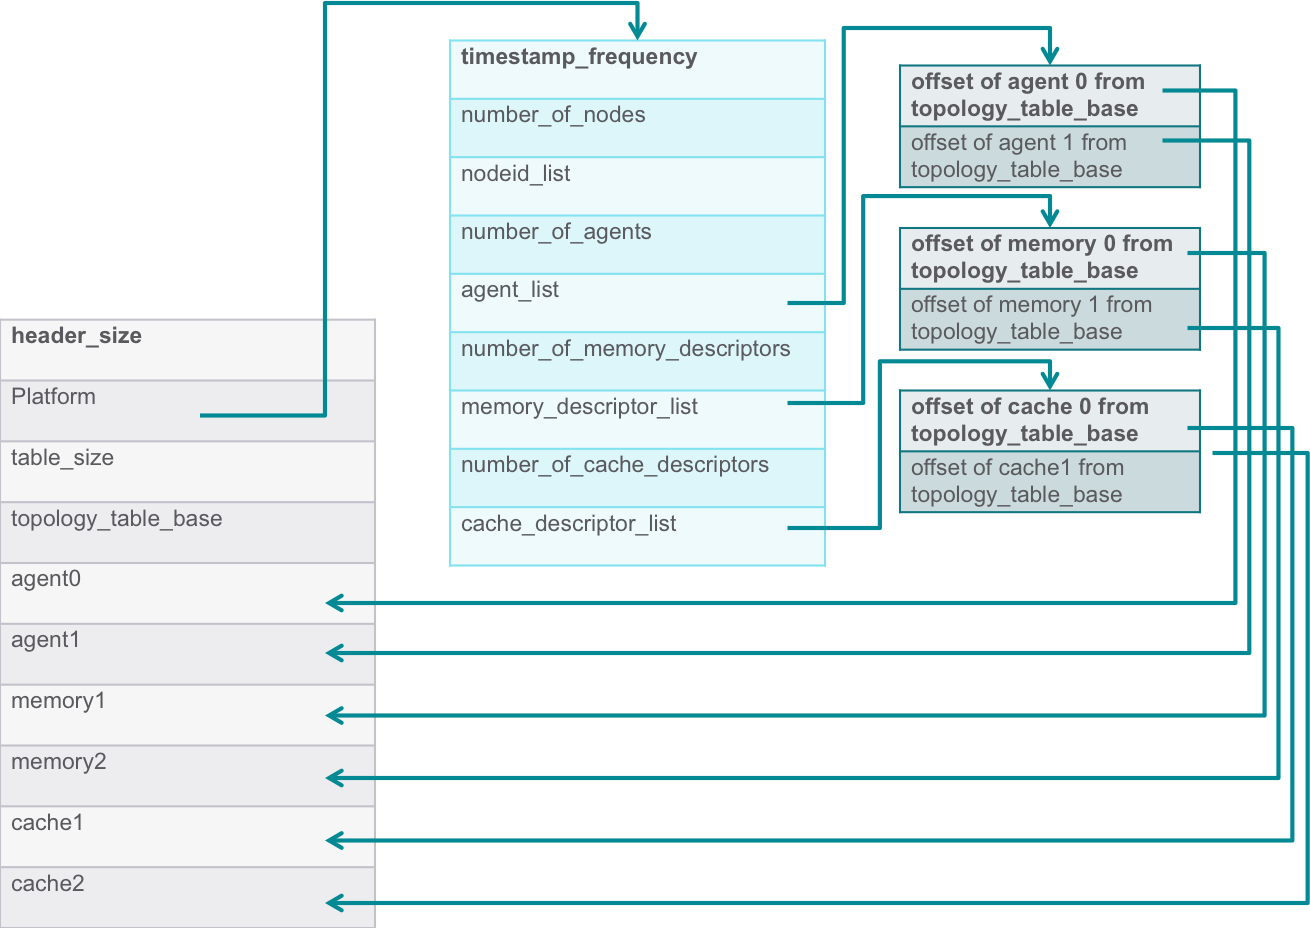
\includegraphics[width=0.5\textwidth]{fig/topologytable}
%   \centering
%   \caption{Structure of the Topology Table}
%   \label{fig:topology_table}
% \end{figure}

% The table structure is shown in Figure~\ref{fig:topology_table}.
% The first entity in the table is a table header. This is the output
% of the \hsaref{hsa_topology_table_create} API, and is defined as:
% \input{api/altlatex/group-topology-header}

\hypertarget{topology_example}{} \subsection{Example}
TODO

\hypertarget{signals}{}\section{Signals}
\label{signals}

In a HSA system, (coherent) global memory can serve as a means for message
passing, asynchronous communication or synchronization between agents. A signal
is an alternative communication mechanism, possibly more power efficient. A
signal carries a value, which can be updated or conditionally waited upon via an
API call or HSAIL instruction.

Signals may be utilized in many ways. For example, a running kernel, after it
finishes producing a part of its computation, may set the signal in the
dependency packet of another kernel dispatch so that the queue processor can
resolve the dependency and launch the second kernel. Signals cannot be used for
Inter-Process Communication.

Signal are represented by opaque signal handlers; signal values are represented
using four or eight bytes, depending on the machine model in use. To put the
signal in error state, the two most significant bits in the signal value are set
and all other bits cleared. It is the users burden to check if an error has
occurred by looking at the return code of the \hsaref{hsa_signal_wait_acquire}
invocation. Any negative value at the signal triggers the
\hsaref{HSA_STATUS_FAILURE} return code from the wait API. A signal that is
already in error may further be decremented to a larger negative value.

\mariotodo{signal creation missing}Once a signal is created for a particular
context, it may be bound to other contexts. This is useful when signal is used
across different components of a users application.

Sending a signal entails updating a particular value at the signal. In addition
to the update of signals using Send, the API for send signal must support other
atomic operations as well: \emph {AND, OR, XOR, Exchange, Add, Subtract,
  Increment, Decrement, Maximum, Minimum} and \emph{CAS}. Each operation on a
signal value has the type of synchronization explicitly included in its
name. For example, Send-Release is a Send on a signal value with Release
synchronization. The set of (action, synchronization) signal modifiers available
in the API match the corresponding HSAIL instructions~\cite{prm}. For
efficiency, a unique signal API has been created for each of these actions.


% Apart from the no synchronization case, which is referred to as \emph{none}
% synchronization, there are three types of synchronization defined in the systems
% architecture requirements:
% \begin{description}[font=\it, leftmargin=1.5em]
% \item[Acquire synchronization] No memory operation listed after the acquire can
%   be executed before the acquire-synchronized operation. Acquire synchronization
%   can be applied to various operations including a load operation.
% \item[Release synchronization] No memory operation listed before the release can
%   be executed after the release-synchronized operation. Release synchronization
%   can be applied to various operations including a store operation.
% \item[Acquire-Release synchronization] This acts like a fence. No memory
%   operation listed before the Acquire-Release synchronized operation can be
%   moved after it nor can any memory operation listed after the Acquire-Release
%   synchronized operation be executed before it.
% \item[Relaxed synchronization] No synchronization is applied to the send or wait
%   operation.
% \end{description}

\begin{description}[font=\it, leftmargin=1.5em]
\item[Acquire-Release synchronization] Exchange, Maximum
\item[Release synchronization] Send, CAS, AND, OR, XOR, Add, Substract, Increment, Decrement
\item[Relaxed synchronization] Send, Exchange, AND, OR, XOR, Add, Substract, Increment, Decrement, Maximum, Minimum
\end{description}

Waiting on a signal returns the current value at the opaque signal object. The
wait has a runtime defined timeout which indicates the maximum amount of time
that an implementation can spend waiting. The signal infrastructure allows for
multiple senders/waiters on a single signal.

The user may wait on a signal, with a condition specifying the terms of
wait. The wait can be done either in the HSA Component via an HSAIL wait
instruction or via a runtime API. Wait \emph{reads} the value, hence Acquire and
Acquire-Release synchronizations may be applied to the read. The synchronization
should only assume to have been applied if the status returned by the wait API
indicates a success (i.e. return value is \hsaref{HSA_STATUS_SUCCESS})

\hypertarget{signal-example}{} \subsection{Example}
TODO

\hypertarget{architected-queue}{} \section{Queues} \label{architected-queue}
HSA hardware supports kernel dispatch through user mode queues. A queue is
associated with a specific component, which might have several queues attached
to it. Two queue types are supported: queues which can consume any kind of AQL
packets (discussed in Section~\ref{AQL}), and service queues. A service queue
consumes agent dispatch packets that are used to specify runtime-defined or user
registered functions that will be executed on the agent (typically, the host
CPU).

Agents write AQL packets to the user mode queue of a particular component. The
queue memory is processed by a packet processor as though it is a ring
buffer. The details on how commands can be written to the queue via AQL packets
are discussed in detail in~\cite{sar}.

The HSA runtime allows the user to create a user mode queue by invoking
\hsaref{hsa_queue_create}, which is responsible for allocating memory to hold
AQL packets. The pointer to the beginning of the allocated memory is stored in
the \reffld{base_address} field. No memory shall be allocated by an
implementation if the queue creation fails. An implementation might not
initialize the queue structure if queue creation fails, so the user should only
rely on the error code returned to determine if the queue is valid.

Internally, the queue structure contains a read index and a write index. Both
indexes are not directly exposed to the user, who can only access them by using
dedicated APIs.  The available index functions differ on the index of interest
(read or write), action to be performed (addition, compare and swap, etc.), and
memory order (relaxed, release, etc.).

The read index is automatically advanced when a packet is read by the packet
processor. When the agent observes that the read index matches the write index,
the queue can be considered empty (it does not mean that the kernels have
finished execution, just that all packets have been consumed). The write index
and the read index never wrap when the write index reaches its maximum value,
but an asynchronous error is generated by the packet processor and the queue is
put in error state.

The \reffld{doorbell_signal} field contains a signal that the agent writing
packets uses to indicate the packet processor that it has work to do. The value
which the doorbell signal must be signaled with corresponds to the identifier of
the packet that is ready to be launched.  The new task might be consumed by the
packet processor even before the doorbell signal has been signaled by the
agent. This is because the packet processor might be already processing some
other packet and observes that there is new work available, so it processes the
new packets. In any case, the agent must ring the doorbell for every batch of
packets it writes.

\mariotodo{clarify service queues}This service queue is configured when a user
mode queue is created. The service queue is visible to HSA agents through the
queue structure \reffld{service_queue} field and is serviced by an appropriate
HSA agent. The application may chose to not use a service queue, select the
runtime managed service queue, or a queue managed by the application. The
address of the service queue associated with the user mode queue is returned in
the queue structure. If there is no associated service queue then the NULL
address will be returned. The API allows different user mode queues to have a
different associated service queue. It also allows for the service queue to be
user managed. The API allows the user to specify that runtime return a default
shared service queue which is created when the runtime is initialized.

\hypertarget{queue-errors}{}\subsection{Queue States} \label{queue-errors}

A queue in HSA, once created, can be in one of the following states:
\emph{active}, \emph{error pending inactive}, \emph{error inactive} or
\emph{destroyed}. A state diagram showing the various states and transitions is
shown in Figure~\ref{fig:queuestate}.

\begin{description}
\item[Active] Once a queue is successfully created using the
  \hsaref{hsa_queue_create} API, it enters the active state. Packets can be
  added to the queue and are consumed by the packet processor. The actual
  initiation of dispatch may depend on the resources available for the
  dispatch. Writing packets to the queue, updating the write index or ringing
  the doorbell have effect only when the queue is in the active state. The queue
  is not monitored by a packet processor in any other state.

\item[Error pending inactive] If an error is encountered during packet
  processing (invalid packet format, wrong signal, etc.) or dispatch, the packet
  processor stops. At this point, there might be in-flight kernels and resources
  (such as segment allocation) that have been setup for a dispatch but have not
  yet been freed. So the queue is not entirely inactive, but once the
  asynchronous activity concludes, it will become inactive. A queue in
  \emph{error pending inactive} state is not to be considered as destroyed, it
  still needs to be destroyed so the runtime can reclaim the memory allocated
  for this queue. If the user provides a callback at queue creation time, the
  callback is invoked after the queue is marked inactive.

\item[Inactive] If all the asynchronous activity concludes, the queue enters the
  inactive state. A queue can also enter this state when the user explicitly
  invokes the \hsaref{hsa_queue_inactivate} API (note that the callback
  implementation for the queue error callback can invoke this API). In an
  inactive state, the queue structure and its packets may be inspected. Only the
  packets that are between the read index and the write index in the queue
  structure are considered to be valid for inspection by the user. The packet
  processor guarantees that all the packets that have been consumed by the
  packet processor (see Section~\ref{dispatch-packet}) will be signaled with
  either the completion information or an error. Inactivating a queue that is
  already is in the inactive state has no effect.

\item[Destroyed] The queue has been destroyed by the user. The resources
  allocated to the queue and the memory for the queue are no longer valid. The
  queue structure is no longer valid.
\end{description}

\begin{figure}
  \centering
  \scriptsize
  \begin{tikzpicture}[auto,on grid,node distance=5cm,state/.style={circle,draw,minimum size=40pt}]
    \node[state]                 (s0) {Active};
    \node[state,dashed,align=center,right=of s0]       (s1) {Error\\Pending\\Inactive};
    \node[state,align=center,right=of s1]       (s2) {Error\\Inactive};
    \node[state,accepting,double distance=1pt,below=3cm of s1]   (s3) {Destroyed};
    \path[->]
    % create edge without defining start node
    (-3,0) edge node {\hsaref{hsa_queue_create}} (s0)

    ([yshift=-.4em]s0.east) edge  node[below] {error in packet} ([yshift=-.4em]s1.west)
    ([yshift=+.4em]s0.east) edge node[above] {error in dispatch} ([yshift=+.4em]s1.west)
    (s0) edge[bend left=20]  node {\hsaref{hsa_queue_inactivate}} (s2)
         edge  node[left] {\hsaref{hsa_queue_destroy}} (s3)

    ([yshift=-.4em]s1.east) edge[dashed]  node[below] {pending kernels complete} ([yshift=-.4em]s2.west)
    ([yshift=+.4em]s1.east) edge[dashed] node[above] {\hsaref{hsa_queue_inactivate}} ([yshift=+.4em]s2.west)
    (s1) edge[dashed]  node[anchor=center,fill=white] {\hsaref{hsa_queue_destroy}} (s3)

    (s2) edge  node[right] {\hsaref{hsa_queue_destroy}} (s3)
         edge[loop right] node[anchor=east,above,yshift=+1.0em,xshift=+1.5em] {\hsaref{hsa_queue_inactivate}} ()
    ;
  \end{tikzpicture}
  \caption{Queue state diagram.}
  \label{fig:queuestate}
\end{figure}


The queue will report packet processing or parsing error, system error,
dependency resolution error, and signaling error (signal destroyed by the time
it needed to be signaled by packet processor).

The queue error reporting infrastructure supports and reports a single error per
queue and attempts to inactivate the queue on the first error it encounters.

\subsection{Example}
TODO

% TODO(mmario): this example is completely wrong
%\lstinputlisting{example/queue.c}


\section{Architected Queuing Language Support}
\label{AQL}\hypertarget{AQL}{}
AQL is a command interface for describing a dispatch or a dependency in a
standard format for the queue packet processor.The HSA API declares structures
for the different types of AQL packets described in~\cite{sar}: always reserved,
invalid, dispatch, agent dispatch and barrier.

\hypertarget{dispatch-packet}{}\subsection{Dispatch packet}
\label{dispatch-packet}

A dispatch packet is used to submit tasks to a HSA component. It can have five
different states: \emph{on queue}, \emph{launch}, \emph{error},
\emph{active} or \emph{complete}. Figure~\ref{fig:packetstate} shows the
different states of a packet and transitions leading to those states.

\begin{figure}[b]
  \centering
  \scriptsize
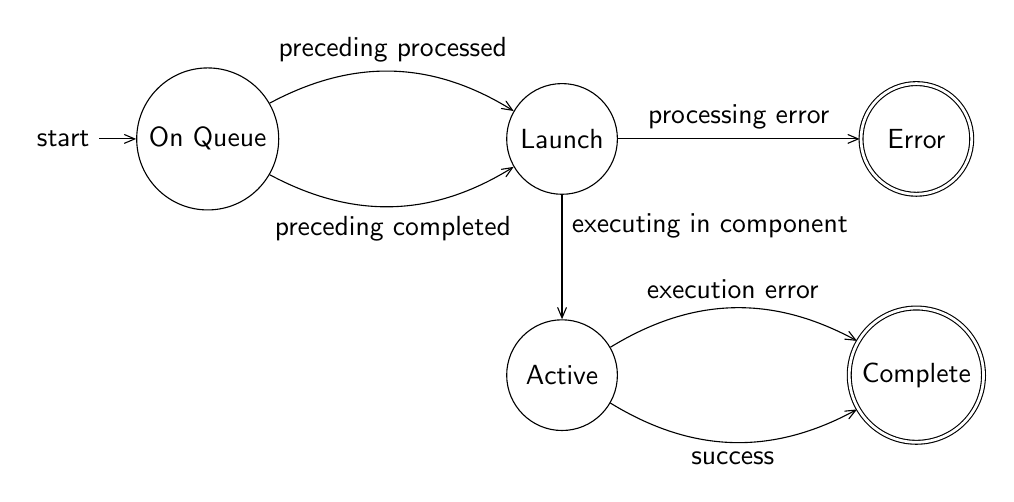
\begin{tikzpicture}
[auto,on grid,node distance=4.5cm,state/.style={circle,draw,minimum size=40pt}]
   \node[state,initial]                 (s0) {On Queue};
   \node[state,right=4.5cm of s0]       (s1) {Launch};
   \node[state,below=3cm of s1]       (s2) {Active};
   \node[state,accepting,double distance=1pt,right=of s1]   (s3) {Error};
   \node[state,accepting,double distance=1pt,right=of s2]   (s4) {Complete};
   \path[->]
     (s0) edge[bend right]  node[below] {preceding completed} (s1)
          edge[bend left] node[above]{preceding processed} (s1)
     (s1) edge  node {processing error} (s3)
          edge  node[near start] {executing in component} (s2)
     (s2) edge[bend right]  node[below] {success} (s4)
          edge[bend left]  node[above] {execution error} (s4)
     ;
\end{tikzpicture}
  \centering
  \caption{Dispatch Packet State Diagram}
  \label{fig:packetstate}
\end{figure}

\begin{description}
\item[On queue] A packet is considered to be in the on queue state once the
  format of the packet is different from
  \hsaref{HSA_AQL_PACKET_FORMAT_ALWAYS_RESERVED} and
  \hsaref{HSA_AQL_PACKET_FORMAT_INVALID}.

\item[Launch] If this dispatch packet has the barrier bit set, then the
  processing of this packet occurs only after all prior kernels have completed
  execution. Otherwise, the processing starts once the preceding packets have
  completed their launch phase.

\item[Error] the packet processor encountered an error processing this
  packet. This results in a queue error (see Figure~\ref{fig:queuestate}) and
  the packet enters the error state (the completion object is signaled with
  error by the packet processor). The following errors are indicated via an
  error signaled to the completion object: processing parsing error, dependency
  resolution error, system error and premature termination due to queue
  inactivation. When the user invokes the \hsaref{hsa_queue_inactivate} API
  or the \hsaref{hsa_queue_destroy} API while the packet is in this state, the
  completion object will be signaled with an error.

\item[Active] If the packet processing is successful and the kernel the
  packet represents is either executing or queued for execution, the packet
  enters the active state. From active state, either successful or failed
  execution both take the packet into the completed state. Alternatively, queue
  inactivation can also take the packet out of active state into complete state.
  When the user invokes the \hsaref{hsa_queue_inactivate} API or the
  \hsaref{hsa_queue_destroy} API while the packet is in this state, the
  completion object will be signaled with an error.

\item[Complete] A packet enters a complete state after its completion
  signal is signaled (either with success or error).
\end{description}

A dispatch packet is considered processed once the packet processor processes it
and makes the queue slot occupied by this packet available. A processed dispatch
packet may endure a period of time where it is awaiting its dispatch on to the
HSA component. Even such packets awaiting execution are still considered as
processed.

\hypertarget{segment-sizes}{}\subsubsection{Segment sizes}
\label{segment-sizes}

If the kernel being dispatched uses private and group segments, the user is
required to specify the sizes of these segments in the dispatch
packet. Manually calculating this information is not feasible and requires
visual inspection of the user program, which itself may have been generated by a
higher-level compiler. Hence the user must rely on the finalizer to get the
corresponding segment sizes. Further details about determining segment sizes are
described in Section~\ref{finalizerchapter}.

Of the other HSA segments, the kernarg segment is also a part of the dispatch
packet, but as a pointer. This is because the kernarg segment carries the
arguments required to execute the kernel being dispatched and must be setup by
the user (the layout of this segment is language/finalization specific and
associated with the code object generated by finalization) prior to writing the
AQL packet to the queue (unlike the group and private segments, whose lifespan
spans only the active state of the dispatch packet). % Please refer to the HSAIL
% service layer \mariotodo{missing} for an example on how to setup the kernarg
% segment for the HSAIL language, which is based on the 32/64 bit modes the kernel
% is compiled in.

\hypertarget{agent-packet}{}\subsection{Agent Dispatch packet}
\label{agent-packet}

Agent Dispatch AQL packets can be used to do dispatches on the agent queue. The
HSA Queue API allows for creation of either agent queues or component queues in
the core API (vendor-specific extensions may support queues that allow both
agent and component dispatches, but it is not a core feature).

\hypertarget{barrier-packet}{}\subsection{Barrier packet}
\label{barrier-packet}

The barrier packet allows the user to specify up to five dependencies as
\hsaref{hsa_signal_handle_t} objects and requires the packet processor to
resolve them before proceeding. The barrier packet is a blocking packet, in that
the processing of the barrier packet completes the packet and its completion
object is signaled. This is unlike a dispatch packet whose completion may occur
at some future time after the packet has finished processing.

If any of the dependent signals have been signaled with a negative value, the
barrier packet is complete, and will indicate failure in its completion
signal. The \reffld{completion_signal} will be signaled with the error value as
discussed in Section~\ref{signals}. If the queue is not already in an error
state (e.g. the job generating the error was processed in a different queue)
then the packet processor should consider the error code on the dependent signal
to indicate an error in the queue itself and subsequently signal the
\reffld{error_signal} in the queue. When all of the dependent signals have been
signaled with the value 0, the \reffld{completion_signal} will be signaled with
the value 0 to indicate a successful completion.

The barrier packet also has a \reffld{barrier} bit that indicates that this
packet may only be processed when all previous packets have been marked as
completed.

The barrier packet can be in one of the following states: \emph{on queue},
\emph{launch}, \emph{completed, error} or \emph{completed,
  success}. Figure~\ref{fig:barrierpacketstate} shows the state transition
diagram.
\begin{figure}
  \centering
  \scriptsize
  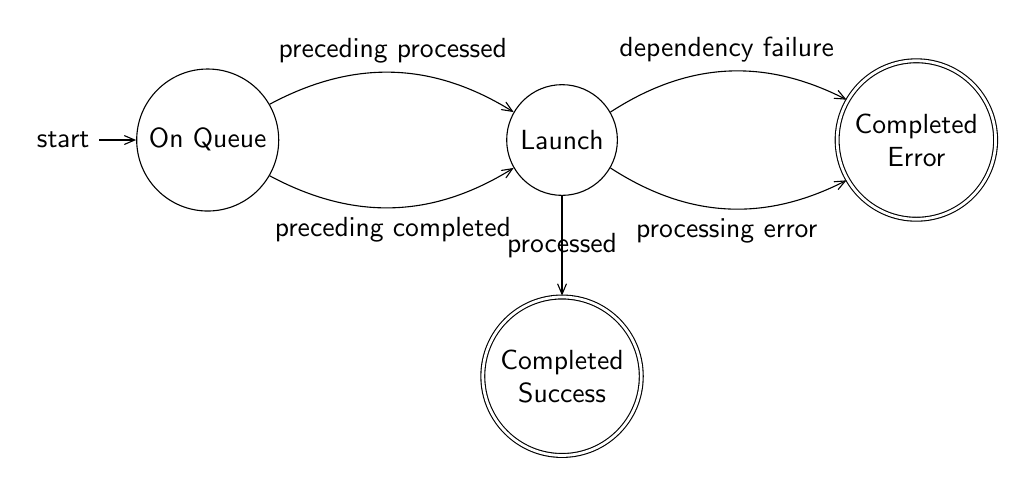
\begin{tikzpicture}[auto,on grid,node distance=4.5cm,state/.style={circle,draw,minimum size=40pt}]
    \node[state,initial]                 (s0) {On Queue};
    \node[state,right=4.5cm of s0]       (s1) {Launch};
    \node[state,accepting,double distance=1pt,align=center,right=of s1]   (s2) {Completed \\Error};
    \node[state,accepting,double distance=1pt,align=center,below=3cm of s1]   (s3) {Completed \\Success};
    \path[->]
    (s0) edge[bend right]  node[below] {preceding completed} (s1)
         edge[bend left] node[above]{preceding processed} (s1)
    (s1) edge[bend right]  node[below] {processing error} (s2)
         edge[bend left] node[above]{dependency failure} (s2)
         edge node[anchor=center] {processed} (s3)
    ;
  \end{tikzpicture}
    \caption{Barrier Packet State Diagram}
  \label{fig:barrierpacketstate}
\end{figure}

\begin{description}
\item[On queue] A packet is considered to be in the on queue state once
  the format of the packet is changed from invalid (a value of 0) to a value of
  1 or 2 or 3. Any other value for format puts the packet and the queue in error
  state.
\item[Launch] If this barrier packet has the barrier bit set, then the
  processing of this packet occurs only after all prior dispatch packets have
  completed execution. Otherwise, once the packets prior to this packet are
  processed, the packet processor begins to process this packet and the packet
  enters the processing state. From the launch state, two states are possible:
  completion, error or completion, success.
\item[Completed with Error] The barrier packet reaches this state from the
  processing state if (a) one of the dependency signals had an error, and (b) if
  the packet was malformed (e.g. bad signal object or invalid usage of reserved
  bits). A barrier packet can also reach this state when the user invokes the
  \hsaref{hsa_queue_inactivate} API or the \hsaref{hsa_queue_destroy} API while
  the packet is in processing state (the completion object will be appropriately
  signaled with an error).
\item[Completed with Success] The barrier packet had all its dependencies met,
  its completion object has been signaled with a value of 0.
\end{description}

\hypertarget{aql-example}{}\subsection{Example}\label{aql-example}
TODO

\section{Memory}\label{memory}\hypertarget{memory}{}

One of the key features of HSA is its ability to share global pointers between
the host application and code executing on the component. This ability means
that an application can directly pass a pointer to memory allocated on the host
to a kernel function dispatched to a component without an intermediate copy.

\hypertarget{memory-registration}{}\subsection{Registration}\label{memory-registration}

When a buffer will be accessed by a kernel running on a HSA device, programmers
are encouraged to register the corresponding address range beforehand by using
the appropriate HSA core API invocation. While kernels running on HSA devices
can access any valid system memory pointer allocated by means of standard
libraries (for example, malloc in the C language) without resorting to
registration, there might be a performance benefit from registering the buffer
with the HSA core component. When an HSA program no longer needs to access a
registered buffer in a device, the user should deregister that virtual address
range by using the appropriate HSA core API invocation.

\input{api/altlatex/group-register}

\hypertarget{registration-usage}{}\subsubsection{Example}\label{registration-usage}

A buffer is registered by indicating its starting address and a size. The size
does not need to match that of the original allocation. For example:

\begin{lstlisting}
void* ptr = malloc(16);
status = hsa_memory_register(ptr, 8);
if(status == HSA_STATUS_ERROR_INVALID_ARGUMENT)
  handle_error(status);
\end{lstlisting}

 is a valid program. On the other hand:

\begin{lstlisting}
void* ptr = malloc(16);
status = hsa_memory_register(ptr, 20);
if(status == HSA_STATUS_ERROR_INVALID_ARGUMENT)
  handle_error(status);
\end{lstlisting}

is not a valid program, because we are registering a range that spans several
allocations, or might not be entirely allocated.

Registrations can overlap previously registered intervals. A special case of
overlapped registrations is multiple registration. If the same interval is
registered several times with different sizes, the HSA core component will
select the maximum as the size of all the registrations. Therefore, the
following program:

\begin{lstlisting}
status = hsa_memory_register(ptr, 8);
if(status == HSA_STATUS_ERROR_INVALID_ARGUMENT)
  handle_error(status);
status = hsa_memory_register(ptr, 16);
if(status == HSA_STATUS_ERROR_INVALID_ARGUMENT)
  handle_error(status);
\end{lstlisting}

behaves identically to this program:

\begin{lstlisting}
hsa_memory_register(ptr, 16);
if(status == HSA_STATUS_ERROR_INVALID_ARGUMENT)
  handle_error(status);
hsa_memory_register(ptr, 16);
if(status == HSA_STATUS_ERROR_INVALID_ARGUMENT)
  handle_error(status);
\end{lstlisting}

While the described behavior might seem counter-intuitive, consider the
following scenario: A pointer is registered twice with different sizes s1 and
s2. When the pointer is deregistered, which interval should be deregistered: (p,
s1) or (p, s2)? If all the registrations of the same pointer are considered
identical by the core runtime, that problem is eliminated.

Deregistering a pointer that has not been previously registered results in an
\emph{info} status indicating the same.

The following code snippet revisits the introductory example. The code is almost
identical to the original, except that we register the buffers that will be
accessed from the device after allocating them, and we deregister all that
memory before releasing it. In some platforms, we expect this version to perform
better than the original one.


\hypertarget{globalmemory}{}\subsection{Global  Memory Allocation}\label{globalmemory}

While a HSA component is capable of accessing pageable system memory by
definition, for scenarios where wants memory allocated that has already been
registered (combine the allocation with memory registration), the HSA runtime
provides an interface, \hsaref{hsa_memory_allocate} to allocate memory that is
internally registered by the runtime:

\input{api/altlatex/group-memory-allocate}

\hypertarget{kernarg}{}\subsection{Kernarg Memory}\label{kernargmem}

The kernarg memory that AQL packet points to (see Section~\ref{AQL}) holds
information about any arguments required to execute AQL dispatch on a HSA
component. While any system memory may be used for kernarg memory,
implementation/platform specific optimizations are possible if HSA core runtime
provided API are utilized for allocating and copying to the allocated kernarg
memory. To facilitate such optimizations, HSA core runtime defines the following
API:

\input{api/altlatex/group-kernargmem}

\hypertarget{device-memory}{}\subsection{Component Local Memory}
\label{device-memory}

Component local memory is a memory type that is dedicated specifically for a
particular HSA component. This memory could provide higher bandwidth for
component access (than system memory) with the limitation that the host might
not be able to access it directly. HSA runtime provides a host interface to
allocate/deallocate and access component local memory.

\input{api/altlatex/group-memory-local}

\hypertarget{device-memory-usage}{}\subsubsection{Example}\label{device-memory-usage}

Component memory is allocated by indicating the size and the HSA device it
corresponds to. For example, the following code allocates 1024 bytes of device
local memory:

\begin{lstlisting}
void* component_ptr = NULL;
hsa_memory_allocate_component_local(1024, component, &component_ptr);
\end{lstlisting}

To access component memory from the host, the user can call
\hsaref{hsa_memory_copy_component_local_to_system} in similar fashion as in
memcpy. This interface allows the user to perform component-to-host memory
copy. For example:

\begin{lstlisting}
 const size_t DATA_SIZE = 1024;
 void* src_ptr = malloc(DATA_SIZE);
 void* dest_ptr = NULL;
 hsa_memory_allocate_component_local(DATA_SIZE, device, &dest_ptr);
 hsa_memory_copy_component_local_to_system(dest_ptr, src_ptr, DATA_SIZE);
\end{lstlisting}

copies 1024 bytes from system to component local memory.

The user should not register or deregister component local memory.


%\hypertarget{coredebug}{}\section{Execution Control}\label{core debug}
% As per the systems architecture specification, the HSA system must support
% debugging of a HSAIL kernel. The HSA Programmers Reference Manual (PRM)
% describes that the debug section could hold debug data and such a section can be
% placed within a function. This allows the high-level compiler that generates
% HSAIL to embed debug specific information. This information makes its way into
% the debug section in the brig. This information can be used for associating a
% HSAIL level instruction to the higher level functionality. In addition to this,
% the PRM also discusses the \refhsl{debugtrap_u32} that halts the current
% wavefront and transfers control to the agent. The single operand to
% \refhsl{debugtrap_u32}, \char`\"{}src\char`\"{} is passed to the agent and can
% be used to identify the trap.

% To support this infrastructure in the runtime, the Core API defines a structure
% that can be used to exchange information between the kernel executing on the HSA
% component and the agent.

% The core runtime defines a structure, mailbox, whose purpose is to exchange
% information as a part of execution control. Mailbox is a synchronous
% communication mechanism between the HSA component and any agents. The HSA
% component indicates a \refhsl{debugtrap_u32} or syscall activity by sending a
% signal indicating it has written to some location in the mailbox. The HSA PRM
% defines:

% \begin{description}
% \item \refhsl{queueactivegroupcount_global_u32} {\itshape dest, address}
%   Returns the maximum number of work-groups that can be executed in parallel for
%   dispatches executed on the User Mode Queue with address.
% \item \refhsl{activegroupid} index that ranges from 0 through
%   \refhsl{queueactivegroupcount_global_u32}-1.
% \end{description}

% The mailbox is an array of structures of size
% \refhsl{queueactivegroupcount_global_u32}. Since \refhsl{activegroupid} is
% always unique within a queue for any concurrent execution of kernels in that
% queue, indexing into the mailbox by different work items happens without
% conflicts. When a workgroup encounters a syscall or a \refhsl{debugtrap_u32},
% the component indexes into its mailbox by accessing it via
% \refhsl{activegroupid} from within the \refhsl{queueptr}. Once the corresponding
% mailbox is accessed, pertinent information (see structure below) for each work
% group is populated.  Subsequently the component sets the full flag, sends a
% signal to agent by accessing the \reffld{mailbox_signal} inside the queue
% structure (see Section~\ref{architected-queue}), and waits for the full flag to
% be emptied. The mailbox structure is defined as follows.
% \input{api/altlatex/group-interrupt-condition}
% \input{api/altlatex/group-execution-info}

% The agent waits on the signal, processes the mailbox, and clears the full
% flag. If this kernel had a debugtrap_u32, a simple check for debugtrap can be
% written the following way:

% \lstinputlisting{example/mailbox-simple.c}

\hypertarget{agent}{}\section{Agent Dispatch}\label{agent}
The core runtime supports agent dispatches from an HSA agent. The
runtime defines a default service queue for every user mode queue created by the
user. This default service queue is available to the HSAIL programs and the user
applications may submit agent dispatch packets to the service queue or any user
mode queue. The service queue shares the same structure as the regular HSA
queue. The default service queues are monitored by the
runtime.


\hypertarget{extensions}{}\section{Extensions to the Core Runtime
  API}\label{extensions}

When an implementor of the core runtime specification is not supporting any of
the extension API, they will return
\hsaref{HSA_STATUS_ERROR_EXTENSION_UNSUPPORTED} as a return status for that API.

Individual vendors may define vendor extensions to HSA core runtime, or multiple
vendors may collaborate to define an extension. The difference is in the naming
scheme used for the symbols (defines, structures, functions, etc.) associated
with the function:

\begin{itemize}
\item Symbols for single-vendor extensions that are defined in the global
  namespace must use the following naming convention:
  \begin{itemize}
  \item \emph{hsa_svext_\textless COMPANY_NAME \textgreater_}. For example,
    a company ``ACME'' defining a single-vendor extension would use the prefix
    \emph{hsa_ext_acme_}. Company names must be registered with the HSA
    Foundation, must be unique, and may be abbreviated to improve the
    readability of the symbols.
  \end{itemize}
\item Symbols for multi-vendor extensions that are defined in the global
  namespace must use the following naming convention:
  \begin{itemize}
  \item \emph{hsa_ext_} For example, if another company embraces extension in
    the example above from Company ``ACME'', the resulting symbols would use the
    prefix \emph{hsa_mvext_}.
  \end{itemize}
\end{itemize}

Any constant definitions in the extension (\#define/enumerations) use the same
naming convention, except using all capital letters. So, using the single-vendor
extension example from above, the associated defines and enumerations would have
the prefix \refenu{HSA_EXT_ACME_}.

The symbols for all vendor extensions (both single-vendor and multi-vendor) are
captured in the file {\bf hsa/vendor_extensions.h}. This file is maintained by
the HSA Foundation. This file includes the enumeration
\hsaref{hsa_vendor_extension_t} which defines a unique code for each vendor
extension and multi-vendor extension. Vendors can reserve enumeration encodings
through the HSA Foundation. Multi-vendor enumerations begin at the value of
1000000. For example, using the examples above, the
\hsaref{hsa_vendor_extension_t} enumeration might be:

\input{api/altlatex/group-vendor-ext}

HSA defines the following query function for vendor extensions:

\input{api/altlatex/group-query-vendorextension}

\subsection{Example}
An example that shows a hypothetical single-vendor extension ``Foo'' registered
by company ``ACME''. The example includes four defines and two API functions.
Note the use of the structure \reftyp{hsa_svext_acme_foo_t} and how this
interacts with the \hsaref{hsa_vendor_extension_query} API call.

\lstinputlisting{example/extension.c}

%%%%%%%%%%%%%%%%%%%%%%%%%%%%%%%%%%%%%%%%%%%%%%%%%%%%%%%%%%%%%%%%%%%%%%%%%%
%%%%%%%%%%%%%%%%%%%%%%%%%%%%%%%%%%%%%%%%%%%%%%%%%%%%%%%%%%%%%%%%%%%%%%%%%%
%An enumeration, \texttt{HsaSignalSyncType} allows the user to specify the
%synchronization type for a particular send or wait operation on a
%signal. It is defined as follows:
%
%\begin{framed}
%  \begin{lstlisting}
%    typedef enum {
%            kHsaNone=0,
%            kHsaAcquire=1,
%            kHsaRelease=2,
%            kHsaAcquireRelease=3
%    }HsaSignalSyncType ;
%  \end{lstlisting}
%
%\diffblock{
%  \begin{description} [font=\tt]
%    \item[kHsaNone] \hfill \\
%            indicates that none of the below synchronization methods
%            are desired
%    \item[kHsaAcquire] \hfill \\
%            acquire, applies to wait and atomic send
%    \item[kHsaRelease] \hfill \\
%            release, applies to send and atomic send
%    \item[kHsaAcquireRelease] \hfill \\
%            applies to send, wait and atomic send
%  \end{description}
%}
%
%\end{framed}

%An enumeration, \texttt{HsaSignalAction} allows the user to
%specify what to do with the \emph{value} in the
%\texttt{HsaSignalSend} API. The enumeration is defined as follows:
%
%\begin{framed}
%  \begin{lstlisting}
%    typedef enum {
%            kHsaSignalSet=0,
%            kHsaSignalAtomicAnd=1,
%            kHsaSignalAtomicOr=2,
%            kHsaSignalAtomicXor=3,
%            kHsaSignalAtomicExch=4,
%            kHsaSignalAtomicAdd=5,
%            kHsaSignalAtomicSub=6,
%            kHsaSignalAtomicInc=7,
%            kHsaSignalAtomicDec=8,
%            kHsaSignalAtomicMax=9,
%            kHsaSignalAtomicMin=10,
%            kHsaSignalAtomicCas=11
%    }HsaSignalAction ;
%  \end{lstlisting}
%\diffblock{
%  \begin{description} [font=\tt]
%    \item[kHsaSet] \hfill \\
%            basic set signal with release, no atomics
%    \item[kHsaSignalAtomicAnd] \hfill \\
%            atomic AND, signal.value \&= value
%    \item[kHsaSignalAtomicOr] \hfill \\
%            atomic OR, signal.value OR= value
%    \item[kHsaSignalAtomicXor=3,] \hfill \\
%            atomic XOR, signal.value XOR= value
%    \item[kHsaSignalAtomicExch] \hfill \\
%            atomic Exch
%    \item[kHsaSignalAtomicAdd] \hfill \\
%            atomic add, signal.value += value
%    \item[kHsaSignalAtomicSub] \hfill \\
%            atomic subtract, signal.value -= value
%    \item[kHsaSignalAtomicInc] \hfill \\
%            atomic increment, signal.value++, value is ignored
%    \item[kHsaSignalAtomicDec] \hfill \\
%            atomic increment, signal.value-, value is ignored
%    \item[kHsaSignalAtomicMax] \hfill \\
%            atomic maximum, MAX(signal.value,value)
%    \item[kHsaSignalAtomicMin] \hfill \\
%            atomic minimum, MIN(signal.value,value)
%    \item[kHsaSignalAtomicCas] \hfill \\
%            atomic compare and swap, if(signal.value == value2)
%            signal.value = value2
%  \end{description}
%}
%\end{framed}

% \input{signal_send_release}
% \input{signal_send_acquire_release}
% \input{signal_and_release}
% \input{signal_or_release}
% \input{signal_xor_release}
% \input{signal_exch_release}
% \input{signal_exch_acquire_release}
% \input{signal_add_release}
% \input{signal_sub_release}
% \input{signal_inc_release}
% \input{signal_dec_release}
% \input{signal_max_none}
% \input{signal_min_none}
% \input{signal_cas_release}

%To just signal using a set (no atomics), action
%\texttt{kHsaSignalSet} may be used. However, only
%\texttt{kHsaRelease} and \texttt{kHsaAcquireRelease} synchronization
%types apply to the \texttt{kHsaSignalSet} action.

%The Table \ref{actionandsync} shows which synchronization operations
%apply to which signal actions. The implementation of the
%\texttt{HsaSignalSend} will return a failure if correct combinations
%are not used.

% \begin{table}[b!]
% \begin{center}
%         \begin{tabular}{|p{3in}| p{3in}|}
%     \hline
%     \textbf{HsaSignalAction} & \textbf{Correponding HsaSignalSyncType that can be
%     used with the action} \\
%     \hline
%     kHsaSignalSet & kHsaRelease, kHsaAcquireRelease \\ \hline
%     kHsaSignalAtomic<And,Or,Xor,Exch, Add,Sub,Inc,Dec,Max,Min,Cas &
%     kHsaRelease, kHsaNone, kHsaAcquire, kHsaAcquireRelease \\ \hline
%   \end{tabular}
% \end{center}
% \caption{Action and Synchronization Combinations}
% \label{actionandsync}
% \end{table}

% \begin{framed}
%   \begin{lstlisting}
%   typedef enum {
%           kHsaSignalConditionEqual,
%           kHsaSignalConditionNotEqual,
%           kHsaSignalConditionLessThan,
%           kHsaSIgnalConditionGreaterThanOrEqual
%   }HsaSignalWaitCondition;
%   \end{lstlisting}
% \diffblock{
%   \begin{description}[font=\tt]
%     \item[kHsaSignalConditionEqual] \hfill \\
%             wait until timeout or value == signal.value
%     \item[kHsaSignalConditionNotEqual] \hfill \\
%             wait until timeout or value $\ne$ signal.value
%     \item[kHsaSignalConditionLessThan] \hfill \\
%             wait until timeout or value \textless  signal.value
%     \item[kHsaSignalConditionGreaterThanOrEqual] \hfill \\
%             wait until timeout or value $\ge$ signal.value
%   \end{description}
% }
% \end{framed}

% In addition to this, the wait API must support \texttt{kHsaRelease}
% and \texttt{kHsaAcquireRelease} synchronizations.

%\begin{framed}
%\lstinputlisting{example/aql_dispatch.c}
%\end{framed}


\chapter{HSA Extensions Programming Guide}

\section{HSAIL Finalization and Linking}
\label{finalizerchapter} \hypertarget{finalizerchapter}{}

The following subsections have to be updated according to the API definitions
introduced in version 0.180 of the specification.


\hypertarget{finalizer}{}\subsection{HSAIL Finalization}\label{finalizer}

\hypertarget{linking}{}\subsection{HSAIL Linking}\label{linking}

% Compilation support in the HSA core runtime comprises of a finalization
% step. The primary functionality of this step is to translate the HSAIL to a
% component specific instruction set and produce a compilation unit. It resolves
% user defined symbols that are not already bound via callbacks provided by the
% user.

% HSA components may support HSAIL natively or may have a native ISA that the
% HSAIL needs to be translated into. However, compilation is a necessary step and
% is required despite a HSA components' native support of HSAIL. This is because
% of two primary reasons:

% \begin{enumerate}
% \item The HSA kernel code objects (accessible via the
%   \hsaref{hsa_compilationunit_code_t} structure, discussed in
%   Section~\ref{finalize:codeobject} ) are an output of the finalization process
%   and required as an input for the AQL dispatch packet; to obtain values from
%   the finalizer for segment sizes etc.\ and also to act as a container for
%   component specific execution information.

% \item In order to support kernel dispatches from the HSA component, the kernel
%   code object must reside in a memory layout specification since dispatches
%   initiated from components are able to use memory operations to get the
%   information necessary for a dispatch.
% \end{enumerate}

% \subsubsection{BRIG and .directive Section}
% The core runtime accepts HSAIL programs coded in the BRIG binary format, as
% defined in the HSA PRM~\cite{prm}, for its finalization process. BRIG is a
% binary format defined by the HSA PRM and includes 5 different sections,
% \emph{.string}, \emph{.directive}, \emph{.code}, \emph{.operand}, and
% \emph{.debug}. More information on these sections is described in Section 19.1
% of the HSA PRM. The core runtime structure that represents a BRIG is named
% \hsaref{hsa_brig_t}. This structure is an in-memory representation of the
% BRIG. It is defined as follows:

% [DELETED CODE]

% Of the different sections in BRIG, the .directive section provides information
% to the finalizer on functions, kernels, and global declarations, etc. The
% symbols in the .directive section have defined placement rules (see PRM for more
% information). For example, immediately after a function or kernel directive,
% BRIG requires the directives that describe the arguments to be in a certain
% order. Return arguments are first, followed by input arguments, followed by the
% directives that apply only to the function or kernel.

% The \hsaref{hsa_brig_t} structure has the base address of the directive
% section. A directive for any symbol is represented using an offset into the
% directive section. HSA core runtime defines a type
% \hsaref{hsa_brig_directive_offset_t} to represent the .directive section
% offset. It is typedef to an unsigned 32 bit integer and is defined by all
% implementations as follows:

% [DELETED CODE]

% There are different types of directives specified in the PRM. Of these, the
% control directives are a means to allow implementations to pass information to
% the finalizer via HSAIL. HSA runtime defines a structure
% \hsaref{hsa_control_directives_t} to represent the values of control
% directives both at finalization time and to record information in the kernel
% code object. Control directives may also be specified within the HSAIL
% code. When conflicting values are specified for a particular directive specified
% in HSAIL and at finalization time, the runtime will do one of the following: (a)
% perform a union (OR operation) when possible (e.g. when the value represents a
% bit field).

% (b) when a union is not meaningful, the runtime will require that the value
% provided at finalization time via the \hsaref{hsa_control_directives_t}
% structure match the value for this directive in the HSAIL kernel.

% The \hsaref{hsa_control_directives_t} structure is defined as
% follows:

% [DELETED CODE]

% Where, the \hsaref{hsa_control_directive_present64_t} is defined as a 64bit
% unsigned integer.
% [DELETED CODE]

% The enumeration \hsaref{hsa_control_directive_present64_t} is a bit set
% indicating which control directives have been specified. It is accessible via a
% mask, \hsaref{hsa_control_directives_present_mask_t}, which is defined as
% follows:

% [DELETED CODE]

% User can choose to either break on exceptions or just detect them. The PRM
% defines the policy to be exception-type specific, i.e.\ different IEEE
% exceptions supported by HSA (see the definition of the enumeration
% \hsaref{hsa_exception_kind_mask_t} below) can be handled with different
% policies (BREAK vs.\ DETECT). The \reffld{enable_break_exceptions} field
% specifies the set of HSAIL exceptions that must have the BREAK policy
% enabled. It is possible that on some systems, enabling exceptions may result in
% lower code performance. If the kernel being finalized has any
% \texttt{enablebreakexceptions} control directives in HSAIL, then the runtime
% performs a union (OR operation) of values specified by this argument with the
% values in HSAIL control directives. If any of the functions the kernel calls
% have an enablebreakexceptions control directive, then they must be equal to or a
% subset of this union.

% [DELETED CODE]

% \subsubsection{Code Objects}\label{finalize:codeobject}

% There are different code objects defined by the runtime specification in support
% of HSAIL: \hsaref{hsa_kernel_code_t}, \hsaref{hsa_compilationunit_code_t}
% and \hsaref{hsa_function_code_t}. All of them are in memory and can be
% relocatable and/or position independent (which indicates that the object can be
% deep-copied to other memory locations for execution). The HSA runtime provides a
% query API to verify if a particular component supports position independent code
% objects (see Section~\ref{topology}).

% The \hsaref{hsa_compilationunit_code_t} is the header for the code object
% produced by the Finalizer and contains information that applies to all code
% entities in the compilation unit.

% Since core runtime does not define a file format container, the core runtime
% provides API to work with HSAIL programs encoded in the BRIG binary format and
% supports generation of code objects that include kernels to be executed in the
% HSA component and binding of unresolved symbols associated with the code object
% generated.

% Finalizer allocates a single contiguous area of memory to hold the generated
% code for all the code objects.

% The structure of this contiguous area is as follows: Starting at offset 0, the
% ``header'' of this contiguous area is defined by the
% \hsaref{hsa_compilationunit_code_t} structure. The
% \hsaref{hsa_compilationunit_code_t} structure in turn contains an offset to
% an array of \hsaref{hsa_code_entry_t}, one entry per code entity that the
% finalizer has produced code for. Each \hsaref{hsa_code_entry_t} variable
% contains an offset to a \hsaref{hsa_*code_t} object that describes that code
% entity (function/kernel/etc).

% [DELETED CODE]

% Every \hsaref{hsa_*_code_t} code objects start with a common header that also
% contains what kind of code object it is. The common header,
% \hsaref{hsa_code_t}, is defined as follows:
% [DELETED CODE]

% A bit set of flags providing information about the code in a compilation
% unit. Unused flags must be 0. The \hsaref{hsa_code_properties32_t} must be
% used as a type for this flag. The values/mask currently supported is defined as
% follows:
% [DELETED CODE]

% The \hsaref{hsa_compilationunit_code_t} structure is defined as
% follows:
% [DELETED CODE]

% Both the \hsaref{hsa_compilationunit_t} and \hsaref{hsa_*_code_t} objects
% can have implementation define data towards the end of the structure. All
% elements in the contiguous location being accessed by offsets enables such
% definition. This also allows the exact position of the various objects in the
% contiguous memory area to be implementation defined as long as memory alignment
% requirements are met.

% Many of the \hsaref{hsa_*_code_t} objects include a size field which is
% required to be set to the size of the structure. This allows forward
% compatibility and allows for structure definitions to change or include
% implementation specific information.

% The \hsaref{hsa_kernel_code_t} is required for all component dispatches and
% is referred to by the dispatch AQL packets placed in the HSA queue. This allows
% an implementation to rely on all such objects being the same size for more
% efficient navigation to the implementation specific data without need to first
% read the object's size field.

% The \hsaref{hsa_kernel_code_t} is the output of
% \hsaref{hsa_finalize_brig} API and is defined as follows.
% [DELETED CODE]

% \subsubsection{Finalize BRIG API}
% The \hsaref{hsa_finalize_brig} API accepts \hsaref{hsa_brig_t} as an input
% and produces relocatable code object in which global and group symbols are bound
% to actual, component recognizable, addresses. A symbol in the finalization step
% can be a variable, a function, image or a sampler. When finalization occurs, a
% \hsaref{hsa_kernel_code_t}, representing the kernel that needs to be executed
% on the component is generated. However, all the symbols referenced in the
% kernel being finalized may not be resolved with the information provided at its
% finalization. User is allowed to define callbacks that can resolve the symbols
% declared in the global segment, with the following signature:
% [DELETED CODE]

% The finalization step, when successfully executed, can have two distinct
% outputs. The first is the compilation unit code object,
% \hsaref{hsa_compilationunit_code_t} which is discussed in
% Section~\ref{finalize:codeobject}. The second output is of type
% \hsaref{hsa_compilationunit_debug_t} which is only generated when the code is
% compiled with a debug option. This debug information is currently implementation
% defined.

% Since the contiguous memory that {\itshape compilationunit_code} represents and
% the memory for {\itshape compilationunit_debug} need to be allocated, the user
% is expected to provide callbacks for memory allocation.

% The callback is required to have the following signature:
% [DELETED CODE]

% Where caller is the opaque pointer passed to the \hsaref{hsa_finalize_brig}
% that is calling back this function. {\itshape byte_size} is the size in bytes
% of the memory to be allocated. {\itshape byte_alignment} is the required byte
% alignment of the memory allocated. Must be a power of 2. {\itshape address} is
% pointer to location that will be updated with address of allocated memory if
% successful, or NULL if not successful. {\itshape return value} is the HSA
% status of the allocation.
% [DELETED CODE]

% HSAIL does not define a set of options that a finalizer needs to specify. To
% ensure portability, \hsaref{hsa_finalize_brig} must not return an error status
% if a given compilation option is not recognized.

% The callback for the allocation of \hsaarg{compilationunit_debug} is optional
% and is required when the user passes in a flag at finalization to generate debug
% information. This callback, when defined, must have the same signature as
% \hsaref{hsa_alloc_t} above.

% \subsubsection{Freeing The Compilation Unit Code/Debug Object}
% The core runtime also provides a corresponding destruction API that destroys the
% compilation unit code and debug objects. This will reclaim all memory used by
% the \hsaref{hsa_compilationunit_code_t} (including the ISA it contains) and
% associated \hsaref{hsa_compilationunit_debug_t}. It will also unregister the
% ISA memory if appropriate.

% [DELETED CODE]

% Note that destroying does not impact any memory segments that may have been
% allocated/reserved for use in a kernel from this object. It merely releases
% resources used to build the object.

% \subsubsection{Serializing and Deserializing a Compilation Unit}

% Because of the opaque nature of what the compilation unit actually represents,
% and in order for the users of the core runtime to build file containers,
% serialization and deserialization API are defined by the core runtime. The
% definition is as follows:

% [DELETED CODE]

\hypertarget{groupmem}{}\subsection{Group Memory
  Usage}\label{groupmem}

% Group memory can be allocated either
% statically when the finalizer is called or dynamically by the user at launch
% time.

% Static allocation is supported as follows:
% \begin{itemize}
% \item The \hsaref{hsa_finalize_brig} routine writes the amount of group memory
%   needed by the finalized ISA to the
%   \hsaref{hsa_code_descriptor_t}.\reffld{workgroup_group_segment_size_byte}
%   field. The group memory usage includes group memory which is statically
%   allocated in the HSAIL kernel, as well as private group memory used by the
%   finalizer. Different HSA implementations might allocate different amounts of
%   group memory.

% \item The user copies the requested group segment usage to the dispatch packet
%   field \reffld{group_segment_size_bytes}.

% \item The packet processor reads the group memory usage field and reserves the
%   required resources at dispatch time.

% \item Statically allocated group memory starts at a segment offset of 0.

% \end{itemize}

% Dynamically allocated group memory allows the user to specify the group memory
% size when the kernel is launched. This is useful to support dynamic group memory
% allocation features supported by languages such as OpenCL. Essentially, the user
% manually calculates the offset for each kernel argument (including the static
% allocation in the calculation) and passes these as arguments to the HSAIL
% kernel. Specifically:

% \begin{itemize}

% \item As above, the \hsaref{hsa_finalize_brig} routine returns the requested
%   static group allocation.

% \item HSAIL will use standard 32-bit arguments (that is, \ttbf{kernarg_u32})
%   to specify group segment offsets. The user is responsible for computing the
%   offset for each group memory argument location. The first argument must start
%   just above the static allocation, so it always has the offset of
%   \reffld{workgroup_group_segment_size_byte} (see
%   \hsaref{hsa_code_descriptor_t}).

% \item After setting the offset for each group memory argument, the user must set
%   the AQL dispatch packet's \hsaref{hsa_aql_dispatch_packet_t}.\reffld{
%     group_segment_size_bytes} field to the total amount of group memory used
%   (static and dynamic allocations).

% \end{itemize}

% See below for an example of setting up dynamic group memory arguments for a
% kernel.  \lstinputlisting{example/group-sample.c}

% Here is the corresponding kernel and usage model:
% \lstinputlisting{example/group-sample-hsail.c}


\section{Images and Samplers}
\label{images} \hypertarget{images}{}

Images in HSA are accessed by an image handle \hsaref{hsa_image_handle_t}. The
image handle references the image data in memory and records information about
resource layout and other properties. HSA decouples the storage of the image
data and the description of how the device interprets that data. This allows the
developer to control the location of the image data storage and manage memory
more efficiently.

The HSA image format is specified using a format descriptor
(\hsaref{hsa_image_format_t}) that contains information about the image channel
type and the channel order. The image channel type describes how the data is to
be interpreted along with the bit size, and image channel order describes the
number and the order. Not all image channel types and channel order combinations
are valid on a HSA agent. All HSA agents have to support a required minimum set
of image formats (see HSA Programmer's Reference Manual). An application can
query image format capabilities using \hsaref{hsa_image_get_format_capability}.

An implementation-independent image format descriptor
(\hsaref{hsa_image_descriptor_t}) is composed of geometry along with the
image format. The image descriptor is used to inquire the runtime for the HSA
component-specific image data size and alignment details by calling
\hsaref{hsa_image_get_info} for the purpose of determining the
implementation's storage requirements.

The memory requirements (\hsaref{hsa_image_info_t}) include the size of the
memory needed as well as any alignment constraints. An application can either
allocate new memory for the image data, or sub-allocate a memory block from an
existing memory if the memory size allows. Before the image data is used, a HSA
agent-specific image handle must be created using it and if necessary, cleared
and prepared according to the intended use.

A HSA agent-specific image handle (\hsaref{hsa_image_handle_t}) is used by the
HSAIL language for reading or writing using HSAIL \refhsl{rdimage},
\refhsl{ldimage} and \refhsl{stimage}
operations. \hsaref{hsa_image_create_handle} creates an image handle from a
implementation-independent image format descriptor and independently allocated
image data that conforms to the requirements provided by
\hsaref{hsa_image_get_info}.

It must be noted that while the image data technically accessible from its
pointer in the raw form, the data layout and organization is agent-specific and
should be treated as opaque. The internal implementation of an optimal image
data organization could vary depending on the attributes of the image format
descriptor. As a result, there are no guarantees on the data layout when
accessed from another HSA agent. The only reliable way to import or export image
data from optimally organized images is to copy their data to and from a
linearly organized data layout in memory, as specified by the image's format
attributes.

The HSA Runtime provides interfaces to allow operations on images. Image data
transfer to and from memory with a linear layout can be performed using
\hsaref{hsa_image_export} and \hsaref{hsa_image_import} respectively. A
portion of an image could be copied to another image using
\hsaref{hsa_image_copy}. An image can be cleared using
\hsaref{hsa_image_clear}. It is the application's responsibility to ensure
proper synchronization and preparation of images on accesses from other image
operations. See HSA System Architecture spec 2.13 for the HSA Image memory
model.

A HSA agent-specific sampler handle (\hsaref{hsa_sampler_handle_t}) is used by
the HSAIL language to describe how images are processed by the \refhsl{rdimage}
HSAIL operation. \hsaref{hsa_sampler_create_handle} creates a sampler handle
from an agent independent sampler descriptor
(\hsaref{hsa_sampler_descriptor_t}).

\section{Component Initiated Dispatches} \label{architected}
\hypertarget{architectedchptr}{}
%% \hyperlink{coreapi}{Core A\-P\-I
Documentation}\hypertarget{coreapi_dtde}{}\section{Component-\/\-Initiated
Dispatch}\label{coreapi_dtde}

Due to architected support for a queue and design of A\-Q\-L,
H\-S\-A supports component-\/initiated dispatch, which is the ability
for a kernel to dispatch a new kernel by writing an A\-Q\-L packet
directly to a user queue. In simple use cases, the A\-Q\-L packet
can be created on the host and passed as a parameter to the kernel.
This eliminates the need to do dynamic memory allocation on the
component, but has the limitation that the problem fanout must be known
at the time the first kernel is launched (so that the A\-Q\-L
packets can be preallocated). H\-S\-A also supports more advanced
use cases where the A\-Q\-L packet is dynamically allocated
(including the memory space for kernel arguments and
spill/arg/private space) on the component. This usage model obviously
requires dynamic component-\/side memory allocation, for both host and
component memory.

Some requirements to do component-\/initiated dispatch\-:

\begin{itemize}

\item Ability to dynamically choose a kernel to dispatch\-: Let us
assume for example that there are three kernels (A, B and C). If the
host launches A, then the user has the choice of launching B or C,
or even A in case of recursion. So, the user should be able to get
the I\-S\-A and segment size (Hsa\-Aql\-Kernel) from the
corresponding B\-R\-I\-G dynamically. \mbox{[}caveat\-: The code
sample here does not show how we can do this. It assumes that the
Hsa\-Aql\-Kernel is being passed as an argument to the parent kernel
(A in this case)\mbox{]}

\item Ability to dynamically allocate memory from the shader\-: We
need to allocate memory for A\-Q\-L\-Packet, different kernel
segments in the A\-Q\-L\-Packet, kernel arguments, and so forth.

\item Ability for a finalizer to identify a default H\-S\-A queue to
write A\-Q\-L\-Packet\-: The H\-S\-A queue information resides in
the runtime layer of the stack. This needs to be exchanged with the
compiler so it can be stored in the global space. This way, when the
compiler sees the queue, it knows where to pick the H\-S\-A queue
information to write the A\-Q\-L\-Packet.

\item Ability to notify the completion of all the
component-\/initiated dispatches on the host\-:

\begin{itemize}
\item The beginning of execution of the child kernel may or may not
wait for the parent kernel's completion. This is determined by the
user and could be algorithm dependent.
\item If the parent (initiated from host) kernel finishes
successfully, it means all kernels it initiated also finished
successfully.
\item To implement this, we need to track the list of kernels
launched from the parent. Change the status of parent to complete,
only if parent and all its child kernels have completed
successfully.
\end{itemize}
\end{itemize}

Implementations that support component initiated dispatches will
need to support these requirements. If the implementation supports
the stated requirements, the following actions will allow a
component to initiate a dispatch\-:
\begin{itemize}
\item The queue and \texttt{hsa\_code\_object\_t} (describing the
kernel to launch) can be passed as arguments to the parent (the one
launched from the host) kernel. If the dispatch is to the same
queue, it is accessible via an HSAIL instruction.
\item If not, get the Hsa\-Aql\-Kernel from the B\-R\-I\-G for the
kernel that is chosen to be dynamically dispatchd.
\item When new work is to be created, the H\-S\-A\-I\-L code would\-:
\begin{itemize}
\item Use the kernel dynamic memory allocator to allocate a new
A\-Q\-L\-Packet.
\item Use inline H\-S\-A\-I\-L to replicate the functionality of the
Hsa\-Init\-A\-Q\-L\-Packet function. We could perhaps provide an
H\-S\-A\-I\-L library to implement this functionality. Recall this
function\-:
\begin{itemize}
\item Copies some fields from the Hsa\-Aql\-Kernel structure (for
example, the kernel I\-S\-A) to the A\-Q\-L\-Packet
\item Uses a host allocator to allocate memory for the kernel
arguments
\item Uses a component allocator to allocate memory for spill,
private, and arg segments
\end{itemize}
\end{itemize}
\item The H\-S\-A\-I\-L knows the signature of the called function
and can fill in the A\-Q\-L packet with regular H\-S\-A\-I\-L global
store instructions.
\item The H\-S\-A queue is architected, so the H\-S\-A\-I\-L can use
memory store instructions to dispatch the kernel for dispatch.
Depending how the user queues are configured, atomic accesses might
be necessary to handle contention with other writers. Note that, if
the queue information is not passed in as an argument, the default
queue can be chosen by the finalizer as it was exchanged earlier
from the runtime layer.
\item We also need to handle deallocation of the kernel arguments
and spill/private/arg space after the kernel completes.
\item On the host, check if the parent has finished. If the parent
has finished successfully, then it means that all the child kernels
have finished successfully too. If the parent or any of the child
kernels failed, an error code will be returned. 
\end{itemize}


Due to architected support for a queue and design of AQL, HSA supports
component-initiated dispatch, which is the ability for a kernel to dispatch a
new kernel by writing an AQL packet directly to a user queue. In simple use
cases, the AQL packet can be created on the host and passed as a parameter to
the kernel. This eliminates the need to do dynamic memory allocation on the
component, but has the limitation that the problem fanout must be known at the
time the first kernel is launched (so that the AQL packets can be
preallocated). HSA also supports more advanced use cases where the AQL packet is
dynamically allocated (including the memory space for kernel arguments and
spill/arg/private space) on the component. This usage model obviously requires
dynamic component-side memory allocation, for both host and component memory.

Some requirements to do component-initiated dispatch:
\begin{itemize}
\item Ability to dynamically choose a kernel to dispatch: Let us assume for
  example that there are three kernels (A, B and C). If the host launches A,
  then the user has the choice of launching B or C, or even A in case of
  recursion. So, the user should be able to get the ISA and segment size
  (Hsa\-Aql\-Kernel) from the corresponding BRIG dynamically. \mbox{[}caveat:
  The code sample here does not show how we can do this. It assumes that the
  Hsa\-Aql\-Kernel is being passed as an argument to the parent kernel (A in
  this case)\mbox{]}

\item Ability to dynamically allocate memory from the shader: We need to
  allocate memory for AQL\-Packet, different kernel segments in the AQL\-Packet,
  kernel arguments, and so forth.

\item Ability for a finalizer to identify a default HSA queue to write
  AQL\-Packet: The HSA queue information resides in the runtime layer of the
  stack. This needs to be exchanged with the compiler so it can be stored in the
  global space. This way, when the compiler sees the queue, it knows where to
  pick the HSA queue information to write the AQL-Packet.

\item Ability to notify the completion of all the component-initiated
  dispatches on the host:

\begin{itemize}
\item The beginning of execution of the child kernel may or may not wait for the
  parent kernel's completion. This is determined by the user and could be
  algorithm dependent.
\item If the parent (initiated from host) kernel finishes successfully, it means
  all kernels it initiated also finished successfully.
\item To implement this, we need to track the list of kernels launched from the
  parent. Change the status of parent to complete, only if parent and all its
  child kernels have completed successfully.
\end{itemize}
\end{itemize}

Implementations that support component initiated dispatches will need to support
these requirements. If the implementation supports the stated requirements, the
following actions will allow a component to initiate a dispatch:
\begin{itemize}
\item The queue and \hsaref{hsa_code_descriptor_t} (describing the kernel to
  launch) can be passed as arguments to the parent (the one launched from the
  host) kernel. If the dispatch is to the same queue, it is accessible via an
  HSAIL instruction.
\item If not, get the Hsa\-Aql\-Kernel from the BRIG for the kernel that is
  chosen to be dynamically dispatched.
\item When new work is to be created, the HSAIL code would:
\begin{itemize}
\item Use the kernel dynamic memory allocator to allocate a new AQL\-Packet.
\item Use inline HSAIL to replicate the functionality of the
  Hsa\-Init\-AQL\-Packet function. We could perhaps provide an HSAIL library to
  implement this functionality. Recall this function:
\begin{itemize}
\item Copies some fields from the Hsa\-Aql\-Kernel structure (for example, the
  kernel ISA) to the AQL\-Packet
\item Uses a host allocator to allocate memory for the kernel arguments
\item Uses a component allocator to allocate memory for spill, private, and arg
  segments
\end{itemize}
\end{itemize}
\item The HSAIL knows the signature of the called function and can fill in the
  AQL packet with regular HSAIL global store instructions.
\item The HSA queue is architected, so the HSAIL can use memory store
  instructions to dispatch the kernel for dispatch. Depending how the user
  queues are configured, atomic accesses might be necessary to handle contention
  with other writers. Note that, if the queue information is not passed in as an
  argument, the default queue can be chosen by the finalizer as it was exchanged
  earlier from the runtime layer.
\item We also need to handle deallocation of the kernel arguments and
  spill/private/arg space after the kernel completes.
\item On the host, check if the parent has finished. If the parent has finished
  successfully, then it means that all the child kernels have finished
  successfully too. If the parent or any of the child kernels failed, an error
  code will be returned.
\end{itemize}

\begin{appendices}

\chapter{HSA API Reference}
% names of the sections here should match those of the programming guide

\section{Common Definitions}
\input{api/altlatex/group-RuntimeCommon}

\section{Initialization and Shutdown}
\input{api/altlatex/group-context}

\section{Errors and Notifications}
\input{api/altlatex/group-status}

\section{Topology Discovery}
\input{api/altlatex/group-topology}
\input{api/altlatex/group-clock}

\section{Signals}
\input{api/altlatex/group-signals}

\section{Queues}
\input{api/altlatex/group-queue}

\section{Architected Queuing Language Support}
\input{api/altlatex/group-aql}

\section{Agent Dispatch}
\input{api/altlatex/group-agent-dispatch}

\section{HSAIL Finalization}
\input{api/altlatex/group-FinalizerCoreApi}

\section{HSAIL Linking (Service Layer)}
\input{api/altlatex/group-HsailLinkerServiceLayer}

\section{Images and Samplers}
\input{api/altlatex/group-images}

\end{appendices}

% inline bibliography for simplicity.
\bibliographystyle{plain}
\begin{thebibliography}{30}

\bibitem{prm}
HSA Foundation.
\newblock{The HSA Programmer's Reference Manual.}
\newblock{Technical report, HSA Foundation, 2013.}

\bibitem{sar}
HSA Foundation.
\newblock {The HSA Platform System Architecture Specification.}
\newblock{Technical report, HSA Foundation, 2014.}

\end{thebibliography}

\end{document}
